\documentclass{article}
%\usepackage[a4paper, total={6in, 8in}]{geometry}
\usepackage{geometry}
 \geometry{
 a4paper,
 total={210mm,297mm},
 left=20mm,
 right=20mm,
 top=-2mm,
 bottom=2mm,
 }
%\usepackage[margin=0.5in]{geometry}

\usepackage{amsmath,amssymb}
\usepackage{ifpdf}
%\usepackage{cite}
\usepackage{algorithmic}
\usepackage{array}
\usepackage{mdwmath}
\usepackage{pdfpages}
\usepackage{mdwtab}
\usepackage{eqparbox}
\usepackage{cite}
%\onecolumn
%\input{psfig}
\usepackage{color}
\usepackage{graphicx}
\setlength{\textheight}{23.5cm} \setlength{\topmargin}{-1.05cm}
\setlength{\textwidth}{6.5in} \setlength{\oddsidemargin}{-0.5cm}
\renewcommand{\baselinestretch}{1}
\pagenumbering{arabic}
\usepackage{ragged2e}
\renewcommand{\baselinestretch}{1.5}

\begin{document}

\textbf{
\begin{center}
{
\large{School of Engineering and Applied Science (SEAS), Ahmedabad University}\vspace{4mm}
}
\end{center}
%
\begin{center}
\large{B.Tech(ICT) Semester IV: Probability and Random Processes (MAT 202) }\\ \vspace{3mm}
\end{center}
}
\begin{itemize}
\item Group No : S$\_$C3
\item Name (Roll No) : Prachee Javiya(AU1841032)\\\vspace{1mm}
\hspace{26mm} Panth Patel(AU1841020) \\\vspace{1mm}
\hspace{26mm} Dhruvil Dave(AU1841003)
\item Project Title: \textbf{The risk of a major nuclear accident: Calculation and perception of probabilities }

\end{itemize}

\section{Introduction}
\subsection{Background}
\begin{itemize}
    \item The whole of this paper is devoted to calculating the risk of a major nuclear accident.  By this we mean a failure initiating core meltdown. The cost of such accidents amounts to €1 per MWh generated. Setting aside the back of an envelope, which lends itself to quick, simple calculations, the paper gives us an insight into the accidents, from both a theoretical and an empirical standpoint. The study reports a probability of a core melt of $5\times10^{-5}$ per reactor year, in other words, a 0.00005 chance of an accident on a reactor operating for one year. (cit 1) Due to the confidentiality of data and limited resources, we would study one nuclear plant operating for 100,000 reactor years, rather than a fleet of 100000 reactors,operating for 1 year(The frequency remains unchanged).The accident in Fukushima was caused by a tsunami (estimated to be 45 feet tall), which was due to the Tohoku earthquake on March 11; a pair of natural disasters that shut down the power and cooling of three nuclear reactors, leading to three nuclear meltdowns, and hydrogen air explosions. We will individually calculate the probabilities of above events and model them to analyse the risk of next possible nuclear accident in Japan.


    \item
    The main purpose of probabilistic safety assessments is not to estimate the probability of an accident on a specific plant or reactor, but rather to detect exactly what may go wrong, to identify the weakest links in the process and to understand the faults which most contribute to the risk of an accident. We will proceed methodically, starting from conditional probability, taking one branch of the tree and studying it deeper, calculating its probability and see how it affects the total probability. For example, Pr(release|melt|cooling system failure|loss of emergency power source|protective wall round plant breached by wave|7.0 magnitude quake). All the possible sequences form an ‘event’ tree, with a series of forks, each branch being assigned a probability.

    \item Inside a nuclear reactor, slow thermal neutrons are bombarded inside the Uranium-235 core which react with the fuel and the Uranium present inside the fuel captures this slow moving electron and goes into an excited state and finally decays into residual, following a chain reaction. But what is the probability that this slow moving neutron reacts with the fuel? This is decided by a physical quantity which is called cross-section measured in barns(b). This quantity defines that with what amount of cross-section does this slow moving neutron reacts with and higher the cross-section, higher the probability of the reaction. This cross-section is measured w.r.t Incident Energy of slow moving neutron. After doing some mathematics and some quantum mechanical derivations, we get that cross-section formula turns out to be $\sigma = \pi \Bar{\lambda}^2 \frac{\Gamma^2}{(E - E_r)^2 + (\frac{\Gamma}{2})^2}$ which is known as a Breit-Wigner Distribution which is a modified form of Lorentz distribution. We can see that there is a peak in the distribution, which corresponds to $E_r$ which is called the Resonance Energy. At this peak we can see that cross-section is maximized which shows that if an incident Neutron is bombarded at this energy, it has a higher chance of reacting with the Nuclei.
\end{itemize}

\subsection{Motivation}
Nuclear Energy, by witnessing the gradual depletion of natural resources, "probably" will become the next primary source of energy in the near future.
Compared to other fuels, nuclear power costs relatively low (eradicating construction costs) and the likelihood of an accident occurring is also low, but when it does, it makes a huge dent in economic and environmental fabric ;a loss costing in billions(Fukushima Daiichi 11 Mar. 2011). The anomalies of the reaction are unpredictable and random which makes it difficult to track them.In today’s global energy environment, nuclear power plant managers need to consider many dimensions of risk in addition to nuclear safety-related risk.  In general we tend to overestimate any risk relating to rare, fearsome accidents. The purpose of this report is to provide an integrated framework for risk prediction as a tool to enhance the accuracy of predicting a major nuclear accident as well as risks associated with them, including core damage frequency. The reactions will be studied thoroughly in order to determine the output which contribute to a nuclear accident and what is the probability of an accident happening due to it . Things can go wrong in ways that we can not even foresee, we must collect data on all potential incidents that lead to the wrongdoing of a nuclear reactor thus creating a probabilistic model that provides a detailed risk analysis. Besides, who wouldn't want to get accurate answers to  universe's randomness?

\subsection{Case Study}
We aim to analyse the data of the the nuclear accident happened in Fukushima Daiichi; March, 2011. Using the data we will determine the probab

%panth tu lakhje aa

% \begin{itemize}
%     \item Problem identification, Identify  performance metric for the selected project.
% \begin{figure}
%     \centering
%   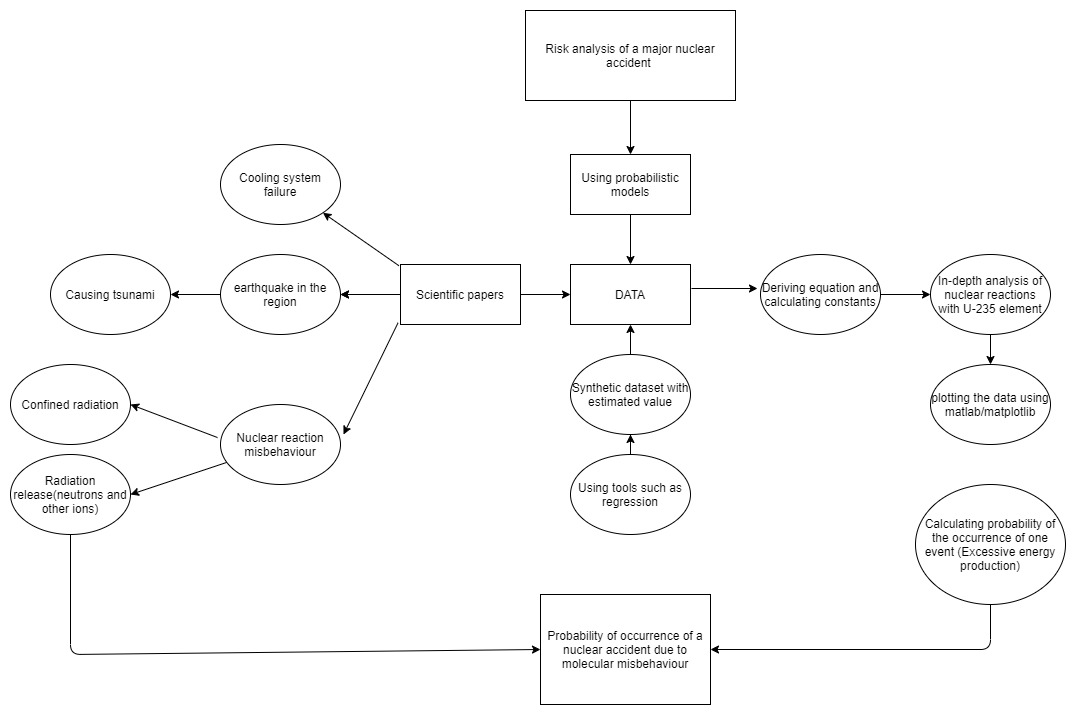
\includegraphics[scale=0.5]{Metric.jpg}
%     \caption{Performance Metric}
%     \label{fig:my_label}
% \end{figure}
% \end{itemize}

\section{Data Acquisition }

\begin{itemize}
    \item Is your Special Assignment Data Dependent? Yes.

    \item \textbf{DD YOUR SECTION niche comment section ma example che}
    If Yes then Define the data acquisition process with complete citation.
\end{itemize}
%are Once accomplished,we can improve sensing performance based on  the knowledge of channel statistics. Further, for more realistic considerations we would extend the above setup to SIMO, MISO and MIMO system models. The performance metrics would be the statistical properties like idle/busy period durations, its mean, variance and Occupancy rate(or duty cycle) of Primary user (PU). The metric for spectrum sensing would be detection probability $(P_d).$ Also the estimation error varies as per sensing period$(T_s)$ and thus KS distance would be an additional metric to be taken into consideration.
	%\vspace{8cm}
\section {Probabilistic Model Used/ PRP Concept Used}
\begin{itemize}

\item Modeling of physical/real-time uncertain Problem, Study of any existing probability based models
\item Include Block/State diagram (If Any)
%\item Explain the probabilistic model used to solve the problem
\item Include the micro/macro level analysis (Identify different scenarios, assumptions, modeling prerequisites etc)
 \begin{itemize}
     \item Application of Conditional Probability to reliability factor :What
follows is a determination of the probability of system failure by the
application of the conditional probability theorem. Figure below is the reference system. It consists of five components arranged on three "success paths. " So long as the components on at least one success path are operating, the system has not failed.\\ \\
    Probability of system failure can be written as : \\\vspace{10mm}
    \hspace{50mm}P(S)=P(S/A)P(A) + P(S/$\Bar{A}$)P($\Bar{A}$)\hspace{30mm} (1)\\
    where\\\vspace{2mm}
    \hspace{15mm}P(S)=Probability of system failure\\\vspace{2mm}
    \hspace{15mm}P(A)=Probability that component A is working (not failed)\\\vspace{2mm}
    \hspace{15mm}P(S/A)=Probability of system failure, given component A has not failed\\\vspace{2mm}
    Probability that a component is working is determined by its failure density function. For now derivation is beyond our scope.We will assume the following equation and move ahead. 
    $$P(\Bar{A})=\int_{0}^{t}f_{A}(t)dt \hspace{30mm} (2)$$
    % \hspace{80mm} (2) \\
    and probability of no failure is \\ \vspace{1mm}
    \hspace{15mm}P($\bar{A}$)=1-P(A)\hspace{30mm} (3)\\
    where,\\ \vspace{2mm}
    \hspace{15mm}$f_{A}(t)$ = failure density function for component A\\
    P(S/A) and P(S/$\bar{A}$) can be calculated by  a stepwise application of the conditional probability theorem to the system shown in Figure.\\ \\
    \textbf{If A has not failed, the system can fail only if components B, C, and D or D or E also fail.}\\\vspace{5mm}
    \hspace{15mm}P(S/A) = P(S/A, B) P(B) + P(S/A,$\Bar{B}$) P($\Bar{B}$)\hspace{30mm} (4) \\
    Since the system will not fail if both A and B are operating then \\\vspace{5mm}
\hspace{15mm}P(S/A, B) = 0 \\ \vspace{5mm}
\hspace{15mm}$\therefore$  P(S/A) =  P(S/A,$\Bar{B}$) P($\Bar{B}$) \\
The probability of system failure given that B has failed is evaluated
as:\\ \vspace{5mm}
\hspace{15mm}P(S/A, B) = P(S/A, $\Bar{B}$, C) P(C) + P(S/A, $\Bar{B}$ , $\Bar{C}$) P( $\Bar{C}$).\hspace{30mm}(5) \\ 
The first term on the right is zero since the system cannot fail if C
has not failed. Equation (5) becomes \\ \vspace{5mm}
\hspace{15mm}P(S/A, $\Bar{B}$) =  P(S/A, $\Bar{B}$ , $\Bar{C}$) P( $\Bar{C}$)\\
The probability of system failure given that C has failed is evaluated
as:\\ \vspace{5mm}
\hspace{15mm}P(S/A,$\Bar{B}$,$\Bar{B}$) = P(S/A,$\Bar{B}$,$\Bar{B}$,D) P(D) + P(S/A,$\Bar{B}$,$\Bar{C}$,$\Bar{D}$) P($\Bar{B}$). \hspace{30mm} (6) \\
We know if that B,C,D fails then the entire system fails. \\
\\ \vspace{2mm}
\hspace{15mm}$\therefore$ P(S/A,$\Bar{B}$,$\Bar{C}$,$\Bar{D}$)=1 \\
Similarly , calculating for E,\\ \vspace{5mm}
\hspace{15mm}\textbf{P(S/A) = [1-P(E)P(D) ] [1-P(C) ] [1-P(B)]}\\

P(S/$\Bar{A}$) can be calculated in the above fashion and it boils down to : \\ \vspace{5mm}
\hspace{15mm}\textbf{P(S/$\Bar{A}$) - [ 1-P(E) P(D)] [l-P(C)]}\\\vspace{5mm}
System failure probability is thus given by :\\\vspace{2mm}
\hspace{15mm} \textbf{P(S) = [1-P(E)P(D)] [1-P(C)][1-P(A)P(B)]}\\
\\
DATA TO BE ADDED YET ACCORDING TO TIME PERIOD.
    \newpage
    \item Distribution of tsunami events triggered by seismic events at a global scale:\\ 
    To describe the earthquake sizes in the target region,a truncated Gutenberg–Richter relationship is adopted:(cite) %https://www.frontiersin.org/articles/10.3389/fbuil.2016.00025/full#B31\\
    $$G(M)=\frac{1-10^{-b(M-M_{min})}}{1-10^{-b(M_{max}-M_{min})}}$$
    where Mmin and Mmax are the minimum and maximum moment magnitudes, respectively.
    For the simulation, it is convenient to convert the continuous distribution of magnitudes into a discrete set of values ($M_{min}$, …, Mi, …, $M_{max}$), assuming that they are the only possible magnitudes; such probabilities are computed as follows:\\
    \begin{center}
        P($M_{i}$)=G($M_{i}$+0.5$ \dot \Delta M$)-G($M_{i}$ - 0.5$ \dot \Delta M$)
    \end{center}
    
where $\Delta M$ is the discretization interval. 
For the analyses, $M_{min}$ and $M_{max}$ are set to 7.375 and 9.125, and a discretization interval of 0.25 is adopted. This means that seven central magnitude values, i.e., 7.5, 7.75, 8.0, 8.25, 8.5, 8.75, and 9.0, are considered to calculate the corresponding conditional probabilities as in the above equation. The minimum magnitude value is chosen, since small-to-moderate earthquakes rarely generate significant tsunamis, and their contributions to the tsunami hazard are negligible. For the Tohoku case study, a b-value equal to 0.9 is adopted(cite2)\\ %https://www.frontiersin.org/articles/10.3389/fbuil.2016.00025/full. 
\\ %https://www3.nhk.or.jp/nhkworld/en/news/backstories/169/
% https://earthquake.usgs.gov/earthquakes/search/
Once the magnitude interval is selected and the major source area containing all possible rupture scenarios is defined, the mean annual rate of occurrence of earthquakes with magnitudes greater than or equal to 7.375 falling in that area can be calculated. Using G-R model with Poisson process for total area,\\
%https://www3.nhk.or.jp/nhkworld/en/news/backstories/169/
Pr(Occurrence of earthquake($>$6.0 $M_{w}$) in Fukushima(70 mile radius) in one) =$\frac{31}{15,798}$  %https://earthquake.usgs.gov/earthquakes/search/  
%https://en.wikipedia.org/wiki/List_of_earthquakes_in_2019
\\
\\
%https://www.frontiersin.org/files/Articles/222571/fbuil-02-00025-HTML/image_m/fbuil-02-00025-g003.jpg   -- add D graph

 \item Radiation leak :\\
 Following a core melt, two possibilities are considered:
either an 8-in-10 chance that radiation will remain confined inside the reactor
containment; or a 2-in-10 chance that part of the radiation will be released into the environment.%http://www.cerna.mines-paristech.fr/Donnees/data08/810-I3WP_13-ME-02_2.pdf
    
    
   
 \end{itemize}
\end{itemize}

\section{Pseudo Code/ Algorithm }
\textbf{DD YOUR SECTION}

\begin{itemize}
    \item Mathematical representation, Algorithm Design/ Pseudo code
\end{itemize}
\section{Coding and Simulation}
\textbf{DD YOUR SECTION }
\subsection{Simulation Framework}
\justify This paragraph must include the values of all controlling parameters set in you simulations, no. of montecarlo iterations, etc.
\subsection{Reproduced Figures}
\begin{itemize}
\item Used Tools (MATLAB, Python, R etc..)
\item Reproduced Figure-1\\
Insert two figures side by side in a same row. The left figure is first figure of your base article (You can crop this). Name this as Figure 1B (Base stands for base article). And the right figure should include the corresponding reproduced figure that you have generated (along with legends). Name this as Figure 1R (R stands for reproduce figure)
Describe the figure in detail(for e.g Figure 1B and 1R shows the plot of $P_d$ versus $P_f$) for different controlling parameters(eg. sample size) and derive the inference.

\item Reproduced Figure-2\\
Follow in the similar way as instructed above. Name the figures as Figure 2R and 2B. \\
Describe the figure in detail and derive the inference.
\end{itemize}

\subsection{New Work Done (Optional)}

\subsubsection{New Analysis}

\subsubsection{New Coding / Algorithm}

\subsubsection{New Results}

\subsubsection{New Inferences}
\begin{itemize}
    \item Describe:
\end{itemize}

Students are advised to share the new derivations with results in correlation with the  reproduce results. Write clear inference for the new results. You are also advised to add new analysis along with the codes.


\section{Inference Analysis/ Comparison}

\begin{itemize}

\item Derive inference-1 from the work.

\item Derive inference-2 from the work.
\end{itemize}

\section{ Contribution of team members}
\subsection{Technical contribution of all team members }
Enlist the technical contribution of members in the table. Redefine the tasks (e.g Task-1 as simulation of fig.1 and so on)
\begin{table}[h]
\centering
\begin{tabular}{|l|l|l|l|l|l|}
\hline
Tasks  & Team member 1 & Team member 2 & Team member 3 & Team member 4 & Team member 5 \\ \hline
Task-1 &               &               &               &               &               \\ \hline
Task-2 &               &               &               &               &               \\ \hline
Task-3 &               &               &               &               &               \\ \hline
\end{tabular}
\end{table}
\subsection{Non-Technical contribution of all team members }
Enlist the non-technical contribution of members in the table. Redefine the tasks (e.g Task-1 as report writing etc.)
\begin{table}[h]
\centering
\begin{tabular}{|l|l|l|l|l|l|}
\hline
Tasks  & Team member 1 & Team member 2 & Team member 3 & Team member 4 & Team member 5 \\ \hline
Task-1 &               &               &               &               &               \\ \hline
Task-2 &               &               &               &               &               \\ \hline
Task-3 &               &               &               &               &               \\ \hline
\end{tabular}
\end{table}


\section{Submission checklist for uploading on Google Drive}
This section provides the submission checklist for smooth and efficient submission process.  (This is for your reference and please remove this while writing your report).
\begin{itemize}

\item Soft copy of this project Report
\item Soft copy of Abstract
\item Soft copy of Concept Map 1 and 2
\item Soft copy of base article
%\item Hard copy of \textbf{turnitin report} (It should be less than 15 percent after excluding the bibliography)
\item Soft copy of analysis (hand written)
%\item Softcopy of above four documents in pan-drive/hard drive.
\item Folder of matlab codes (with proper naming)
\item Folder of reproduced results in .fig and .jpg format
%\item .pdf Scanned copy of analysis (handwritten)
\item latex (.tex) file of the project report.
\end{itemize}
%\vspace{0.5cm}

\bibliographystyle{IEEEtran}
\bibliography{ref.bib}

\end{document}
